\chapter{Preleminaries}
\section{Example}
The same example will be used on many places throughout this report. By explaining the example in detail here, the explanations that use it should be clearer to the reader.

Imagine a Bank that manages different bank accounts which can be identified by their name. Customers can deposit and withdraw money from their accounts by using the ATMs. The customers interact with the ATM through some kind of user interface. This user interface will be implemented in different ways (textual or graphical), depending on our use case (\figref{fig:example_class_diagram}). All operations on the bank account will be dispatched from the ATM to the bank. 

To make the example more interesting, we will some times assume that BANK accesses the network, file system and a database. This will make capture and replay of the system more difficult. %TODO: wahrscheinlich sollten wir das ins Klassen-diagramm nehmen?
%TODO: anmerken, dass die Klassen und methodennamen an Eiffel Styleguide angepasst sind, aber die gleichen Namen auch fuer die Java Beispiele verwendet werden.

 \begin{figure}[ht]
   \centering
   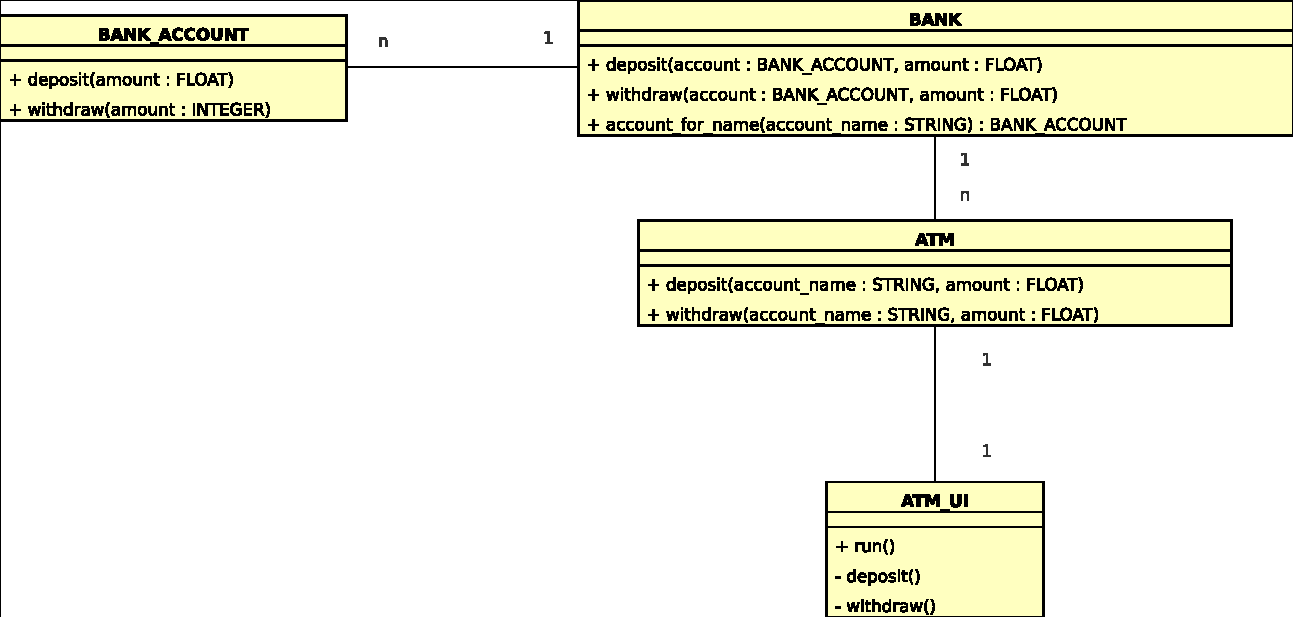
\includegraphics[width=1\textwidth]{illustrations/example_class_diagram}
   \caption{Class Diagram of the Example}
   \label{fig:example_withdraw_sequence}
 %\includegraphics{illustrations/capture_and_replay_generic_structure}
\end{figure}

One use case is money withdrawal by a customer via the ATM. The customer launches the withdrawal operation on the ATM\_UI. The request is passed through the ATM to the BANK which then withdraws the money from the Account. The sequence diagram (\figref{fig:example_withdraw_sequence}) should clarify how the classes interact with each other.

\begin{figure}[ht]
   \centering
   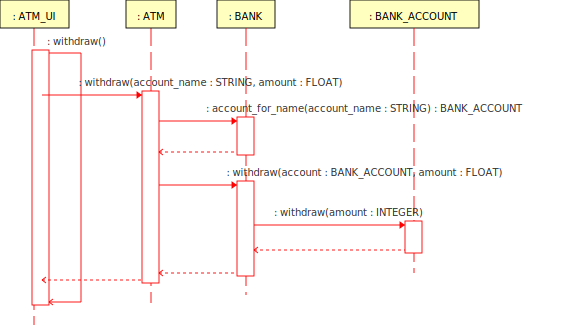
\includegraphics[width=1\textwidth]{illustrations/example_withdrawal}
   \caption{Withdrawal Operation Invoked by the User}
   \label{fig:example_class_diagram}
 %\includegraphics{illustrations/capture_and_replay_generic_structure}
\end{figure}

\section{Selective Capture and Replay}
After giving a short overview about the different capture and replay techniques, our choice will be described here in detail. This chapter summarizes papers from Joshi and Orso about the Java implementation of Selective Capture and Replay (SCARPE) \cite{orso05may, orso06}.

\subsection{Technique and Terminology}
\begin{figure}[ht]
  \centering
  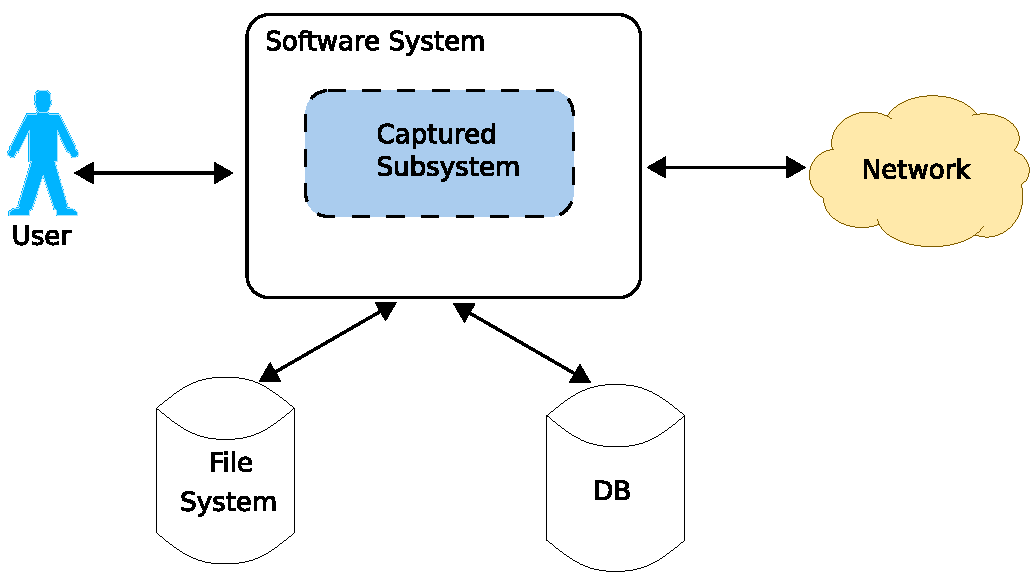
\includegraphics[width=1\textwidth]{illustrations/scr_overall_schema}
  \caption{System Layout of the Example Application (derived from \cite{orso05may})}
  \label{fig:scr_overall_schema}
%\includegraphics{illustrations/capture_and_replay_generic_structure}
\end{figure}
This technique lets the user choose the subset (\emph{captured subsystem}) of the program that should be captured and replayed (\figref{fig:scr_overall_schema}). The technique then only captures the execution data of that subsystem, ignoring the other parts of the system. The relevant interactions between the captured subsystem and the outside world is captured in terms of events; those events are read during the replay phase in order to replay the corresponding interactions. Only a part of the information that traverses the border between the captured system and the rest of the system is captured. This is significant improvement over other existing techniques, especially when big datastructures are passed over the border, but only a part of those datastructures is actually accessed.

\begin{description}
	\item [The observed set] is the subsystem that was selected for capture and replay.
	\item [The observed classes] are the classes in the observed set. Observed code is defined analogous.
	\item [Observed methods and fields] are the fields and methods of the observed classes.
\end{description}
\emph{Unobserved set},  \emph{unobserved classes}, \emph{unobserved code}, \emph{unobserved methods} and \emph{unobserved fields} are the analogous terms for the part of the system that was not selected for capture and replay.
\begin{description}
%	\item [External code]  Nur definieren, wenn es auch gebraucht wird.
	\item [Unmodifiable classes] are the classes whose code can not be modified (e.g. some system classes such as \texttt{java.lang.Class}) due to constraints from the Java Virtual Machines
	\item [Modifiable classes] are all classes except the \emph{unmodifiable classes}
\end{description}

The technique is divided in two main phases: capture and replay. \figref{fig:scr_capture_replay_phase} illustrates the structure of of these two phases in selective capture and replay.
\begin{figure}[ht]
  \centering
  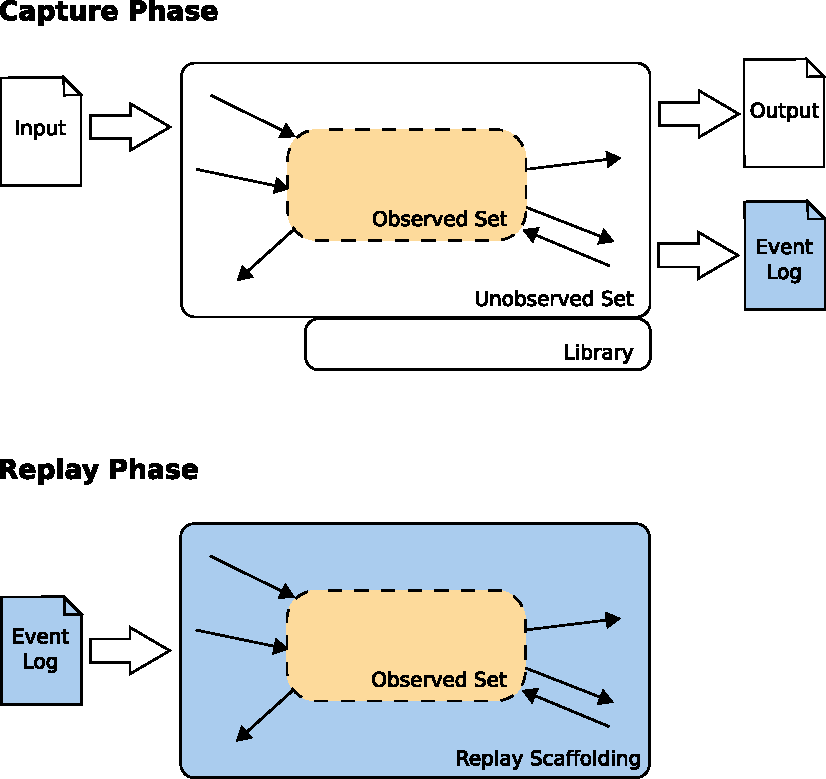
\includegraphics[width=0.8\textwidth]{illustrations/scr_capture_replay_phase}
  \caption{Capture and Replay Phase in Selective Capture and Replay}
  \label{fig:scr_capture_replay_phase}
%\includegraphics{illustrations/capture_and_replay_generic_structure}
\end{figure}
The \emph {capture phase} takes place when the application is run for recording. Before the application starts, the boundaries of the observed set are identified and the application is instrumented in order to be able to capture interactions between the observed set and the rest of the system. While the application runs, the instrumentation generates the events for these interactions and writes them to the \emph{event log}.

In the \emph{replay phase}, the technique generates the \emph{replay scaffolding}. The replay scaffolding uses the event log to replay the events on the observed set. Replaying consists both of performing actions on the observed set (e.g. invocation of a method of the observed set) and consuming actions of the observed set (e.g. receiving a method invocation originally targeted to the unobserved set). Thus the replay scaffolding acts both as a driver and stub.

\subsection{Capture Phase}
%Capture Phase
\subsubsection{Capturing Partial Information}
The technique for capturing only partial information instead of the whole data that flows into unobserved set, selective capture and replay needs an \emph{object ID}. The object ID uniquely identifies a class instance. SCARPE introduces the object ID into the program by adding an additional field to all modifiable classes. It further instruments the creation constructors of these classes so that the unique object ID is aquired from a global counter. For unmodifiable classes however, a reference map is needed to store the object ID of its instances. The object ID for instances of unmodifiable classes is acquired when it is looked up the first time. The reference map uses weak refences so that the referenced objects can be collected by the garbage collector to avoid memory leaks.

Instead of completely recursively serializing the data that crosses the boundaries of the observed set, selective capture and replay only records a small part:
\begin{itemize}
 \item Scalar values (values of a basic type) are fully captured.
 \item For Objects, the technique only captures the object ID and the type, which is necessary to restore the object again during replay phase.
\end{itemize}

To see the advantages of this approach clearer, consider the case when \class{BANK} tries to find out the time of the last log entry of the \class{ATM}. Assume that the classes \class{BANK} and \class{BANK\_ACCOUNT} belong to the observed set and the rest of the application belongs to the unobserved set. The following instructions access the atm's log and print the time of the last log entry:
\javalisting
\begin{lstlisting}
 ATM_LOG log = atm.log
 print (log.time_of_last_entry)
\end{lstlisting}
\class{ATM\_LOG} could contain a thousand of log entries. In the traditional approach, due to the access to the log, the whole data structure including all log entries would be serialized each time the log is accessed. With the approach of selective capture and replay, only the log's object ID and type is written to the event log, as well as another method call to an unobserved class due to the call to time\_of\_last\_entry. This reduces the size of the event loge significantly, because only the the data that is used needs to be written down.

Although this powerful approach is amazingly simple, it is not always easy to grasp. Here is a short reasoning why it works:
\begin{enumerate}
  \item [1)] Instances of observed classes are fully populated during replay, because all actions from the unobserved set are replayed on them and the actions from the observed set are executed as in the original run.
  \item [2)] During replay, observed code accesses to methods or fields can either return objects from instances of observed classes or from instances of unobserved classes.
  \item [3)] When an object of an observed class is returned, it is fully populated due to 1) and therefore its fields and methods can safely be accessed.
  \item [4)] When an object of an unobserved class is returned, each further access to a field or method from observed code to that object would result in the capturing of another boundary crossing event. Therefore the results of these accesses can be reconstructed during replay.
  \item [5)] Therefore, it is assured that during replay, it is possible for the observed code to access the fields and methods like it did in the original run.
\end{enumerate}



\subsubsection {Interactions between Observed and External Code}
Method calls are the basic way to communicate between observed and external part of the application. The technique captures calls in both directions: from observed to unobserved code and vice versa. The events that are captured related to method calls are:

\begin{description}
 \item  [OUTCALL] events that represent calls from observed to unobserved code.
 \item [INCALL] events that represent calls from unobserved to observed code.
 \item [OUTCALLRET] events for the return from outcalls
 \item [INCALLRET] events for the return from incalls
\end{description}

OUTCALL and INCALL events (\emph {call events})  have the same attributes:

\begin{description}
 \item [Receiver] The receiver object
 \item [Method called] Signature of the called method.
 \item [Parameters] The list of scalar values and objects passed to the method.
\end{description}

Capturing of call events involves capturing of scalar values and objects. They are written to the log as follows:

\begin{description}
 \item [Scalar values] are directly written to the log.
 \item [Objects] are written by storing their type and object ID. For null values, the object ID is set to zero. 
\end{description}

OUTCALLRET and INCALLRET events (\emph{callret events}) have only one attribute: the returned value.

OUTCALL and OUTCALLRET events are captured by instrumenting the observed code. A probe is added to all calls to external methods. It is not always possible to distinguish calls to observed code from calls to unobserved code, as we will discuss later.

To capture INCALL and INCALLRET events, proxy methods are introduced in a way that it is not necessary to instrument external code. It is ensured that calls inside the observed code don't call these proxy methods but the actual methods.

Field Accesses are another source of interaction between observed and external classes. Read accesses from unobserved to observed code don't influence the execution behaviour of the observed code therefore they are not captured. Thus three kinds of events are recorded:

\begin{description}
 \item [OUTREAD] events are generated when observed code reads the content of an unobserved field.
 \item [OUTWRITE] events denote write accesses from observed code to unobserved code.
 \item [INWRITE] events are write accesses from unobserved code to observed code.
\end{description}

OUTREAD, OUTWRITE and INWRITE have the same attributes:

\begin{description}
 \item [Receiver:] The object whose field is accessed.
 \item [Field Name:] The name of the field that is accessed.
 \item [Value] The read or written value.
\end{description}

OUTREAD, OUTWRITE events are captured by adding probes in the observed code to accesses to fields of external classes. INWRITE events are captured in the same way, but here the unobserved code is instrumented whenever an observed field is written. Here, the same problem as with OUTCALL evens arises: It is not always possible to determine whether an observed or unobserved field is accessed.

Exceptions are another interaction mechanism that needs to be considered for capture and replay. Because exceptions were not implemented in our Eiffel implementation of selective capture and replay, they will be treated only briefly. For Exceptions, to more types of events were introduced:
\begin{description}
 \item [EXCIN] events are for exceptions that propagate from the external to the observed code.
 \item [EXCOUT] events are for exceptions that propagate from the internal to the external code.
\end{description}
EXCOUT events are captured by wrapping all observed methods with a \texttt{try-catch} block. By wrapping instructions that call an observed method with an exception handler,  EXCIN events are captured.

\subsection{Replay Phase}
During the replay phase, the observed code is reexecuted based on the event log that was gathered during the capture phase. Before replaying the observed code, selective capture and replay instruments the code based on the interactions between observed and external code. 

\subsubsection{Object Creation}
In the replay phase, object ID's are treated in a different way. Now it is necessary to find the object that matches a given object ID, not inverse. In order to allow this resolving, the technique uses a reference map that maps the object ID to all available  objects. The technique extracts the object ID's from the events attributes and then retrieves the associated object or creates it. How these objects are created depends on whether they are instances of observed or external classes.
\begin{description}
 \item [Instances of External Classes] For external classes, \emph{placeholder objects} are created. These objects have the correct type in order to support reflection in the observed code, but their state is irrelevant. After creation, the objects are registered in the reference map.  %placeholder constructors are not that important for us --> no need to describe them...
 \item [Instances of Observed Classes] Instances of observed objects are either created automatically by the observed code or there must be an INCALL event to the constructor in the event log. When replaying an ICALL to a constructor, an entry for the object is entered into the reference map.
 \item [Null Values] If the object ID is zero, null is returned.
\end{description}

%---
\subsubsection{Events Replaying}
For the replay phase, a scaffolding is generated that imitates the behaviour of the external code, thus behaves both as a driver and stub. Whenever control returns tho the scaffolding, it checks whether the received event matches the next event in the log. If the events don't match (\emph{out of sync events}), a message is displayed to the user, who can chose whether do ignore the discrepacy and continue, or stop the replay.  Out of sync events can only occur, if the code was changed between capture and replay phase, for example because the technique is used for regression testing. If the events from log and replay match, the event in the log is  consumed and replay continues.

In contrast to INCALL, INWRITE, OUTREAD, OUTCALLRET and EXCIN, which are necessary to replay the observed code correctly, OUTCALL, INCALLRET, OUTWRITE, EXCOUT are not necessary to replay the observed code, but they can be used as oracles for regression testing. %XXX is this really correct??? I can't imagine that they can guess the object ID's without these events!!!

\begin{description}
 \item [INCALL Events] To replay INCALL events, the method first retrieves the target object from the reference map. If the target object is not in the reference map, it must be either a call to a constructor or a static call. Then, it retrieves the parameters from the reference map, or creates the scalar values corresponding to the parameters. If the object can't be retrieved from the reference map, a placeholder object is created. Then, the technique can call the specified method with all arguments; the control flows to the observed code. 
 \item [INCALLRET Events] INCALLRET events are not essential for replaying the observed code. They occur as a result of INCALL events and are consumed by the replay scaffolding. To ensure a correct replay, the scaffolding checks if returned value conforms to the next event in the event log.
 \item [OUTCALL Events] All invocations to unobserved methods from the observed code are replaced by two instructions: (1) The call to a special feature in the scaffolding (\texttt{consumeCall}) and (2) The assignment of the result of the invocation. For example \texttt{TIME t = atm\_log.time\_of\_last\_entry()}, with TIME and ATM\_LOG both being in the package \texttt{foo}, would be replaced by the following instructions:
\begin{lstlisting}
 Object tmp = scaffolding.consumeCall("foo/ATM_LOG",
                /*object ID for atm_log*/,
                "time:()Lfoo/TIME",
                /*empty array of parameters*/);
 TIME t = (TIME) tmp;
\end{lstlisting}
The scaffolding checks whether type, parameters, target and methodname of the next event from the log matches to the reported call. If everything is allright, then replay continues with the next event, otherwise an error is reported to the user.
 \item [OUTCALLRET Events]As these events occur as a result of OUTCALL events, they are treated within \texttt{consumeCall}. The method looks up return value in the event log and retrieves it using the reference map. 
 \item [OUTREAD and OUTWRITE Events] To replay these events, accesses to unobserved fields are instrumented in the observed code, by calling specific methods of the scaffolding, \texttt{consumeRead} for OUTREAD events and \texttt{consumeWrite} for OUTWRITE events. For example the instruction \texttt{ATM\_LOG = atm.log}, with ATM\_LOG and ATM both belonging to package \texttt{foo}, would be replaced by the following instruction:
\begin{lstlisting}
 ATM_LOG log = scaffolding.consumeRead ("foo/ATM",
                /*Object ID for atm*/,
                "val")
\end{lstlisting}
The methods from the scaffolding control if the events from the log match the detected ones. The method \texttt{outRead} furthermore returns value associated with the event.
 \item [INWRITE Events] In order to replay an INWRITE event, the scaffolding retrieves the target, the name of the field that should be modified and the value to be assigned. It resolves the target, which must exist unless it is a static field access. The value to be assigned is resolved as well or created if it does not exist yet. Finally the scaffolding sets the field of the target to the specified value.
 \item [EXCIN and EXCOUT Events]  To replay EXCIN events, the method \texttt{consumeCall} creates and throws a corresponding exception. This is possible, because EXCIN events can only occur during an outcall. EXCOUT Events are caught by the replay scaffolding and compared to the next event in the event log. If the exception matches the event from the event log, replay continues.
\end{description}

\subsubsection{Assumptions}
%no direct access from unmodifiable classes to a field of an observed class
%no direct access from native code to an observed field
%multi threading does not affect behaviour of the observed code.
%runtime exceptions occur deterministically.
\subsubsection{Special Cases}
%Polymorphism and Dynamic Binding
%Inheritance
%Reflection
%Access Modifiers
%Garbage Collection
%Finalize